\documentclass[tikz,border=4pt]{standalone}
\usepackage{amsmath}
\begin{document}
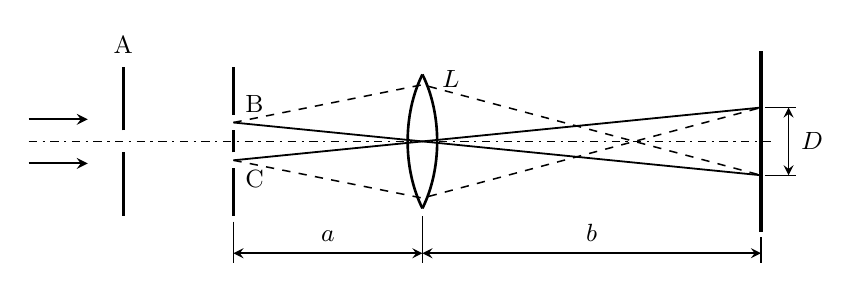
\begin{tikzpicture}[>=stealth, thick, scale=1.0]
  % Optical axis
  \draw[dash dot, line width=0.5pt] (-1.2, 0) -- (8.25, 0);

  % Incident light arrows
  \draw[->, line width=0.75pt] (-1.2, 0.28) -- (-0.45, 0.28);
  \draw[->, line width=0.75pt] (-1.2, -0.28) -- (-0.45, -0.28);

  % Single slit A (top view: two bars with gap at y=0)
  \draw[line width=1.1pt] (0, 0.14) -- (0, 0.95);
  \draw[line width=1.1pt] (0, -0.14) -- (0, -0.95);
  \node[above, font=\small] at (0, 0.98) {$\mathrm{A}$};

  % Double slit B, C at x = 1.4
  \draw[line width=1.1pt] (1.4, 0.34) -- (1.4, 0.95);
  \draw[line width=1.1pt] (1.4, -0.14) -- (1.4, 0.14);
  \draw[line width=1.1pt] (1.4, -0.34) -- (1.4, -0.95);
  \node[above right, font=\small] at (1.42, 0.24) {$\mathrm{B}$};
  \node[below right, font=\small] at (1.42, -0.24) {$\mathrm{C}$};

  % Convex lens at x = 3.8, height L (from -0.85 to +0.85)
  \draw[line width=0.95pt] (3.8, 0.85) .. controls (4.05, 0.35) and (4.05, -0.35) .. (3.8, -0.85);
  \draw[line width=0.95pt] (3.8, 0.85) .. controls (3.55, 0.35) and (3.55, -0.35) .. (3.8, -0.85);
  \node[above right, font=\small] at (3.92, 0.55) {$L$};

  % Screen at x = 8.1
  \draw[line width=1.1pt] (8.1, -1.15) -- (8.1, 1.15);

  % Chief rays through center of lens from B (1.4, 0.24) and C (1.4, -0.24)
  % Magnification in diagram: (8.1-3.8)/(3.8-1.4) = 4.3/2.4 = 1.79 -> image at y = +-0.43
  \draw[line width=0.65pt] (1.4, 0.24) -- (8.1, -0.43);
  \draw[line width=0.65pt] (1.4, -0.24) -- (8.1, 0.43);
  % Marginal rays from B and C to edges of lens
  \draw[line width=0.55pt, dashed] (1.4, 0.24) -- (3.8, 0.72) -- (8.1, -0.43);
  \draw[line width=0.55pt, dashed] (1.4, -0.24) -- (3.8, -0.72) -- (8.1, 0.43);

  % Image spacing D on screen
  \draw[line width=0.5pt] (8.15, 0.43) -- (8.55, 0.43);
  \draw[line width=0.5pt] (8.15, -0.43) -- (8.55, -0.43);
  \draw[<->, line width=0.6pt] (8.45, -0.43) -- (8.45, 0.43);
  \node[right, font=\small] at (8.48, 0) {$D$};

  % Distances a and b along bottom
  \draw[line width=0.5pt] (1.4, -1.02) -- (1.4, -1.55);
  \draw[line width=0.5pt] (3.8, -0.95) -- (3.8, -1.55);
  \draw[line width=0.5pt] (8.1, -1.22) -- (8.1, -1.55);
  \draw[<->, line width=0.6pt] (1.4, -1.42) -- (3.8, -1.42);
  \node[above, font=\small] at (2.6, -1.40) {$a$};
  \draw[<->, line width=0.6pt] (3.8, -1.42) -- (8.1, -1.42);
  \node[above, font=\small] at (5.95, -1.40) {$b$};
\end{tikzpicture}
\end{document}
